%\documentclass[draft]{ws-procs11x85}
%\documentclass[square]{ws-procs11x85}
\documentclass{ws-procs11x85}
\usepackage{color}
\usepackage{graphicx}
\usepackage{subfigure}
\usepackage{wrapfig}
\usepackage{multirow}
\usepackage{url}
\usepackage{titlesec}
\usepackage{wrapfig}
\usepackage{algorithm}
\usepackage{algorithmic}

\newcommand{\tk}[1]{{\bf {\textcolor{magenta}{#1 -- TK}}}}

\newcommand{\hg}[1]{{\bf {\textcolor{red}{#1 -- HG}}}}

\newtheorem{define}{Definition}
%\renewcommand{\baselinestretch}{0.98}

\long\def \ignoreme#1{}
\newcommand{\goodgap}{
        \hspace{\subfigtopskip}
        \hspace{\subfigbottomskip}
}


\begin{document}

\title{Paper Title}

\author{Haitham Gabr, Alin Dobra and Tamer Kahveci$^*$}

\address{CISE Department, University of Florida,\\
Gainesville, FL 32611, USA\\
E-mail: \{hgabr, adobra, tamer$^*$\}@cise.ufl.edu}

\begin{abstract}
Here should come the abstract.
\end{abstract}

\keywords{keyword 1; keyword 2; keyword 3;}

\bodymatter

\section{Introduction} 
\label{introduction}

Studying interactions between proteins has been of utmost importance in
understanding how proteins work collectively to govern cellular
function\cite{schwikowski,uetz}. Such collection of interactions among
proteins is called a protein interaction network. Mathematically, a protein
interaction network is often modeled as an edge-weighted undirected graph where
each node denotes a protein and each edge represents an interaction between a
pair of proteins. The weight of an edge denotes the level of confidence that
this interaction truly exists.

One of the key outcomes of computational analysis of protein interaction
networks is identification of signaling pathways. A signaling pathway is a
series of proteins in which each protein participates in transmitting
biological information by modifying its successor through an
interaction. Thus, signaling pathways can be viewed as simple paths in protein
interaction networks\cite{kelley}.

The confidence value of an interaction between two proteins is often
considered as the probability that a signal is transmitted between
those two proteins.  Thus, the probability that a signal moves through
a pathway is the product of the confidence values of its constituting
interactions. Under this model, Scott et al. conjectured that a signal
tends to move through the most probable pathway~\cite{scott}. They
showed that such pathways yield signaling pathways, and thus help in
reconstructing signaling networks. Following defines the problem of
identifying the most probable pathway in a protein interaction
network.

\paragraph{Problem} Consider a protein interaction network $(V, E, \lambda)$ where
$V$ denotes the set of proteins, $E = \{(u, v) | u,v \in V\}$ denotes the set of
interactions, and the function $\lambda(): E \Rightarrow [0, 1]$  denotes interaction
confidence for each interaction in E. Assume that we are given a set of starting
proteins $S \subseteq V$ and a set of target proteins $T \subseteq V$. Given a
path length denoted by a positive integer $m$, the problem is to find a simple
path $\Phi = v_1 \rightarrow v_2 \rightarrow \ldots \rightarrow v_m$, where
$\prod_{i=1}^{m-1} \lambda(v_i, v_{i+1})$ is maximum among all paths with $v_1 \in
S$, $v_m \in T$ and $v_i \in V \forall i \in \{1, 2, \ldots , m\}$.

The problem above is equivalent to finding a simple path $\phi = v_1
\rightarrow v_2 \rightarrow \ldots \rightarrow v_m$, where
$\sum_{i=1}^{m-1} -$log $\lambda(v_i, v_{i+1})$ is minimum among all
paths with $v_1 \in S$, $v_m \in T$ and $v_i \in V \forall i \in \{1,
2, \ldots , m\}$. The traveling-salesman problem is polynomial-time
reducible to this problem\cite{scott}; therefore it is NP-hard. They
developed a method using a technique devised by Alon et
al.\cite{alon}, called \textit{color-coding}. The basic idea of this
method is to randomly assign each node in the graph one of $m$
different colors, and search for an optimal pathway in the restricted
domain of colorful pathways. A pathway is colorful if and only if all
of its nodes are in different color. Finding a colorful path is
computationally much cheaper than finding a path without assigning
colors. The drawback is that the optimal path may not be colorful in a
random color assignment. If that happens, the color coding method
fails to find the true optimal result. To deal with this, color coding
method repeats the coloring process for several iterations.  The
confidence in the optimality of the result monotonically increases
with each iteration until it reaches a given level of confidence that
the unknown optimal pathway was among the colorful ones in at least
one of these iterations. As we elaborate later in section
\ref{background}, the confidence value depends solely on the pathway
length $m$ and does not capitalize on readily available information
such as the network topology and color assignment. As a result, the
method provides a theoretically correct but very conservative
confidence value.  Hence it requires many iterations in order to
achieve a given confidence level, leading to an unnecessarily
innefficient running time performance.

G{\"u}lsoy et al.\cite{gulsoy} presented an enhanced color-coding
technique called \textit{k-hop coloring}. A colored network is k-hop
colorable if the shortest path between all pairs of same-color nodes
is more than $k$ hops in length. This method exploits the network
topology and the node colors to assign the network a maximal value $k$
such that the network is $k$-hop colorable.  This additional piece of
information allows for higher success probability at each iteration,
yielding fewer iterations than that by Scott et al. However,
subnetworks with high connectivity quickly diminish the ability to
$k$-hop color the whole network for large values of $k$. For example,
a network containing a clique of size $m$ cannot be colored with
($m-1$)-hop coloring using $m$ colors\cite{gulsoy}.

\paragraph{Contribution} In this paper, we consider the problem of
finding signaling pathways in protein interaction networks. We develop
a new coloring method that overcomes the bottlenecks of exisiting
coloring methods by Scott et al.\cite{scott} and G{\"u}lsoy et
al\cite{gulsoy}. Our contribution comes from a deeper understanding of
the relation between network topology, random color assignment and
confidence value. We assign a $k$ value to each node individually by
studying the colors of all the nodes in the network. The $k$ value of
a node $v$ at an iteration indicates that there is no other node $u$
that is reachable from $v$ in $k$ hops such that both $u$ and $v$ have
the same color. For each node, the $k$ value is the largest integer
that satisfies the above constraint. Thus, different nodes in the
network may have different $k$ values. We also study how this reflects
on the resulting success probability for each iteration. Given
different $k$ values for each node on a pathway, we show how to obtain
a bound on success probability.

Based on these findings, We present a new method for detecting signaling
pathways in protein interaction networks using an enhanced k-hop coloring
technique. Given the parameter pathway length $m$, we start by randomly
assigning one of $m$ colors to each node in the graph, we then extract the
optimal colorful pathway. We then calculate our new bound on success
probability. We repeat this process until the cumulative success probability is
at least equal to a given confidence level. Although our theoretical findings
are based on assuming the knowledge of the $k$ values assigned to the unknown
global optimal pathway, we empirically demonstrate that the local optimal
pathway extracted from the domain of colorful pathways yields correct
confidence values.

The coloring methods developed by G{\"u}lsoy et al.\cite{gulsoy} and Scott et
al.\cite{scott} yield special cases of our method. The first method is our
method in the special case of all the nodes in the network having the same $k$
value. The second method is our method in the special case of all the nodes in
the network having $k$ value $= 0$. Hence, our method is guaranteed to perform
at least as good as both of them in these special cases, and better in the
general case.

We provide validation experiments to test the biological significance of our
results. We use \textit{weight p-value} and \textit{functional enrichment} as
validation measures. We also compare the performance of our method against the
one presented by Scott et al.\cite{scott} with respect to how fast our method
reaches a given confidence level as opposed to theirs.

The rest of the paper is organized as follows. Section 2 discusses the
background and related work. Section 3 explains how to obtain a tighter bound on
success probability and describes our enhanced k-hop coloring method. Section 4
shows the experiments performed and their results. Section 5 is the conclusion
of the paper.


\section{Background}
\label{background}

A number of methods have been developed so far to identify signaling networks
from protein interaction networks. These methods differ in the way they
formulate the problem. Among them, Zhao et al.\cite{zhao} formulated a linear
optimization problem that finds the maximum weighted subnetwork with a given
size. The main difference of this approach from this paper is that it is
concerned with finding signaling subnetworks rather than linear pathways.
Kelley et al.\cite{kelley} detected conserved signaling pathways between
related organisms by performing global alignment between their protein
interaction networks. They scored each pathway in terms of the probability of
true homology between aligned pair of proteins, as well as the probability of
true interactions between pairs of proteins along the pathway. Shlomi et
al.\cite{shlomi} introduced QPath, a method for querying protein interaction
networks for pathways using known homologous pathways as queries. They scored
results based on their similarity to the query, number of insertions and
deletions used, as well as the reliability of their interactions. Both Kelley
et al.\cite{kelley} and Shlomi et al.\cite{shlomi} are comparative methods.
They require knowledge of multiple interaction networks. Thus, they solve a
related, yet different, computational problem than the one considered in this
paper.

Lu et al.\cite{lu} presented a divide-and-conquer algorithm to find signaling
subnetworks in protein interaction networks. They recursively partitioned the
network into two sets of vertices, enumerated substructures present in each
set, and then built larger subnetworks from them. They assumed that all edges
have the same weight. They scored the resulting subnetworks based on the
similarity of expression profiles of their nodes to the given source and
destination nodes. This method formulates a different objective. It aims to
detect paths whose proteins are highest in expression similarity, and thus it
does not utilize the confidence in the interactions.

Steffen et al.\cite{steffen} studied detecting signaling pathways in protein
interaction networks as guided by expression data. They listed all pathway
candidates in a protein interaction network using exhaustive search. They
scored each candidate based on how similar the expression profiles of its
genes are. Bebek et al.\cite{bebek} presented a method called PathFinder for
finding new signaling pathways using association rules of known ones. They
started with mining association rules for known pathways, guided by the
knowledge of functional annotations of their proteins. They then performed an
exhaustive search for candidate pathways. From these candidates, they selected
the ones having at least a certain number of the known association rules and an
average interaction weight above a given threshold. The drawback of both of
these methods is that the time complexity of exhaustive graph search is
exponential in terms of the network size, and hence is very inefficient.

Gitter et al.\cite{gitter} presented a method for discovering signaling
pathways by adding edge orientation to protein interaction networks. They
selected an optimal orientation of all edges in the network that maximizes the
weights of all satisfied length-bound paths. They say a path is satisfied if it
follows the same direction along its edges from a source node to a destination node.
They proved that this problem is NP-hard. They provided two approximation
algorithms for it based on available solution methods for weighted Boolean
satisfiability, and a third algorithm based on probabilistic selection. As
shown in their results, these methods do not scale well with increasing the
number of source and destination nodes and the required path length.

The closest studies to that presented in this paper are those by Scott et
al.\cite{scott} and G{\"u}lsoy et al\cite{gulsoy}. The former detected signaling
pathways in protein interaction networks using color coding. The latter
developed topology-aware color coding for network alignment. We describe both
methods in detail in section \ref{introduction}. Both methods run multiple 
coloring iterations. Let us denote the probability that the coloring at an
iteration is successful (i.e. true optimal path is colorful) with $P_s$. The
probability that at least one out of $r$ iterations is successful is $1 - (1 -
P_s)^r$. Following from this, in order to insure confidence of at least
$\epsilon$ ($0 \leq \epsilon \leq 1$), they run $r$ iterations, such that $1 -
(1 - P_s)^r \geq \epsilon$. Both methods calculate success probability as
\begin{equation}
P_s = \frac{m!}{N_c}
\label{ps}
\end{equation}
where $N_c$ is the number of coloring assignments possible for the optimal
pathway. They differ in the way they compute $N_c$. Scott et al.\cite{scott}
calculated $N_c = m^m$. G{\"u}lsoy et al.\cite{gulsoy} calculated a bound $N_c
\leq (m - k)^{m - k} \prod_{i=0}^{k-1} (m - i)$ where $k$ is the value assigned
to the network such that it is $k$-hop colorable. Notice that in equation
\ref{ps}, smaller values for $N_c$ are desirable. This is because small values
for $N_c$ increase success probability, and thus reduces the number of
iterations needed to attain a given confidence level $\epsilon$. This paper
develops a novel method that computes a much smaller upper bound on $N_c$ than
both Scott et al. and G{\"u}lsoy et al., hence a better lower bound on $P_s$.

\section{Method description}

\tk{Rewrite blue stuff below}

{\color {blue}
In this section, we start by properly formulating the problem and
defining common terms that we use in our methods. We then present new
thoughts about pathway detection using color coding. We study the
opportunity of more involving of network topology in our calculation
to obtain a better success probability, and hence needing less number
of iterations and improving performance. Last, we present an enhanced
color-coding method for detecting pathways in protein interaction
networks.
}


\subsection{An overview of our method}

Consider a weighted undirected graph $G = (V, E, w)$, a path length
$m$, a set of starting and target nodes $S$ and $T$ respectively, with
$S, T \subseteq V$.  Scott et al. has shown that it is possible to
find the minimum weight path of a $m$ nodes from $S$ to $T$ in $G$
using dynamic programming~\cite{scott}. As we discussed in detail in
Section~\ref{background}, they use color coding to provide the result
faster, but with uncertainity. They limit uncertainty by computing a
confidence in the result. In principle, our method follows the same
steps. Algorithm~\ref{alg1} presents our method at a high level.

\begin{algorithm}[tbhp]
\caption{Computing the minimum weight path}
\begin{algorithmic}[1]
  \REQUIRE {Input network $G = (V, E, w)$, starting and target node
    sets $S \subseteq V$ and $T \subseteq V$} 
  \REQUIRE {Color set $C = \{c_1, c_2, \ldots, c_m\}$}
  \REQUIRE {Confidence cutoff $\epsilon$}
%\ENSURE {Return distribution table of number of events}
\STATE $P \leftarrow 0$
\COMMENT {Initialize overall success probability}
\WHILE{$P < \epsilon$}
   \STATE {Assign colors to the nodes in $V$ randomly from the set $C$}
   \STATE {$\Phi \leftarrow$ Find the minimum weight colorful path of length $m$ in $G$}
   \STATE Store $\Phi$ in the min-heap of solutions observed so far if it is a new solution.
   \STATE {Compute the probability of success $P_s$ for the current coloring iteration.}
   \STATE {$P \leftarrow 1 - (1 - P)(1 - P_s)$}
   \COMMENT{Update the overall success probability}
\ENDWHILE
\end{algorithmic}
\label{alg1}
\end{algorithm}
%   \COMMENT {blah blah}


The algorithm works iteratively. At each iteration we randomly color
the network (Step 3). We then use dynamic programming to find the
minimum weight colorful path (Step 4). The dynamic programming works
as follows. For any node $v \in V$, a set of colors $C' \subseteq C$ and a
coloring function $c(): V \Longrightarrow C$ denoting the colors assigned to
nodes in $V$, the minimum weight of a colorful path colored only using $C'$,
starting within $S$ and ending at $v$, can be dynamically tabulated using the
following recurrence\cite{scott}:
\begin{equation}
W(v, C') = \min_{u:c(u) \in (C' \backslash \{c(v)\})} W(u, C' \backslash
\{c(v)\}) + w(u, v), |C'| > 1
\end{equation}
where $W(v, \{c(v)\}) = 0$ if $v \in S$ and $\infty$ otherwise. Once we
find the best colorful path in that iteration, we store it in a
min-heap (Step 5). We then compute the probability that the current
iteration was successful in finding the optimal path (i.e., minimum
weighted path regardless of being colorful or not) (Step 6) and update
our confidence in the best result seen so far (Step 7).

As we noted earlier, Algorithm~\ref{alg1} is very similar to the
method by Scott et al.~\cite{scott}. So, a legitimate question is what
is the big challenge addressed in this paper? The answer lies in Step
6 of the algorithm where we compute the probability of success at each
iteration. This step is missing in all the color coding methods to the
best of our knowledge, including Scott et al.~\cite{scott} among
others~\cite{alon, shlomi, dost, gulsoy}. 

 All these existing
methods precompute a probability of success prior to the iterations
and use the same probability value, which is $m!/m^m$, throughout the
iterations (see Equation~\ref{ps}). As a result, they make massive
worst case assumptions that has to hold regardless of which node gets
which color. Our contribution is to eliminate those worst case
assumptions and recompute the probability of success by carefully
inspecting the colors of all the nodes. We explain how we do this in
the next sections.



\subsection{Basic definitions and model}


\begin{wrapfigure}{r}{0.40\textwidth}
  \centering
  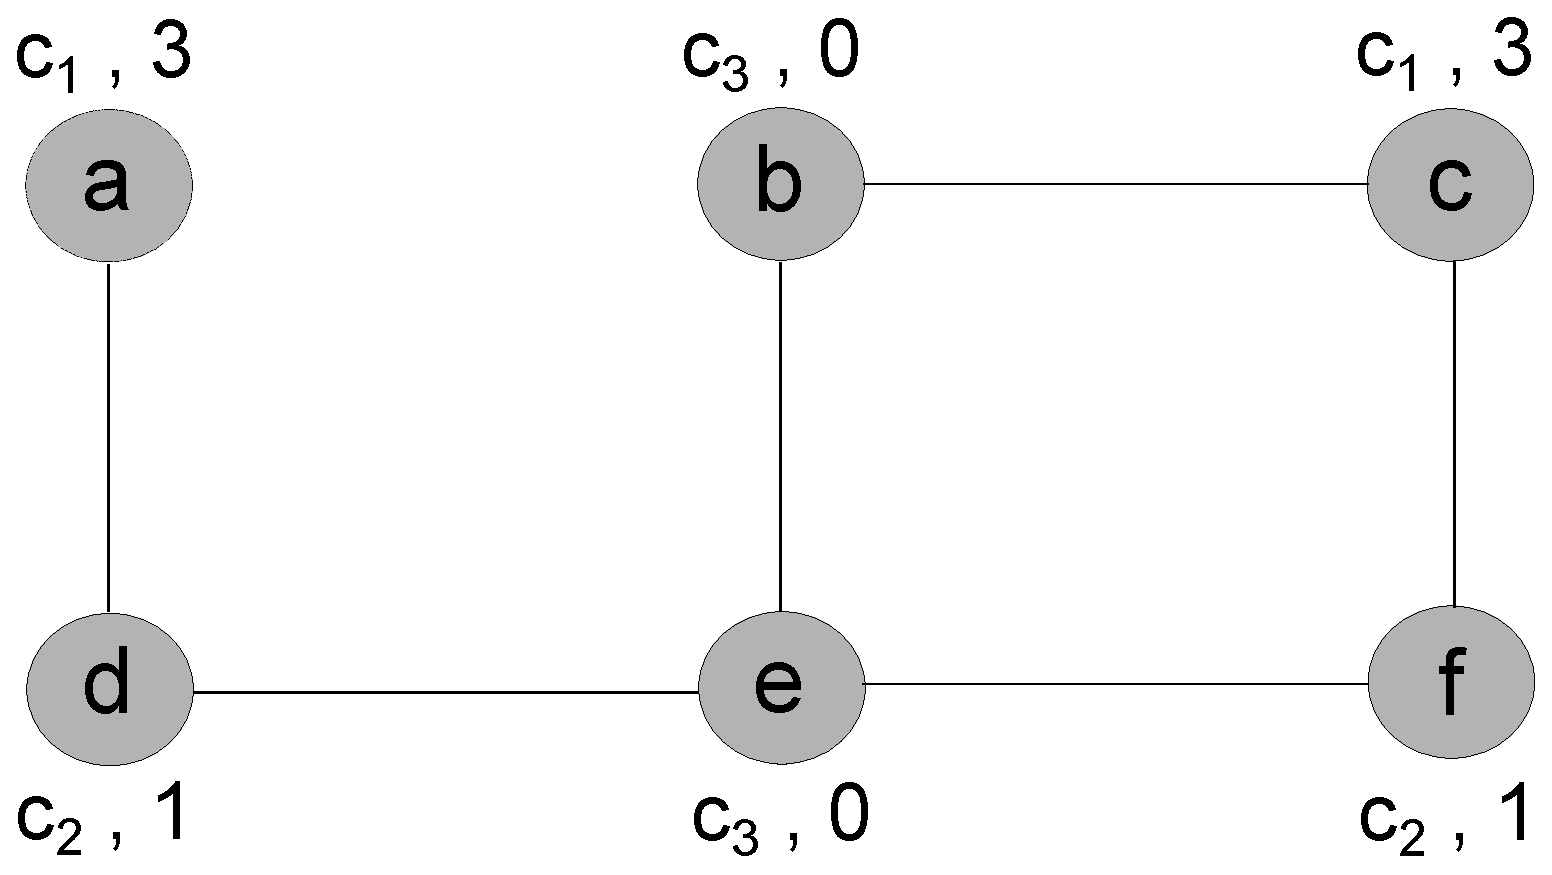
\includegraphics[width=0.35\textwidth]{figures/colors}
%\centerline{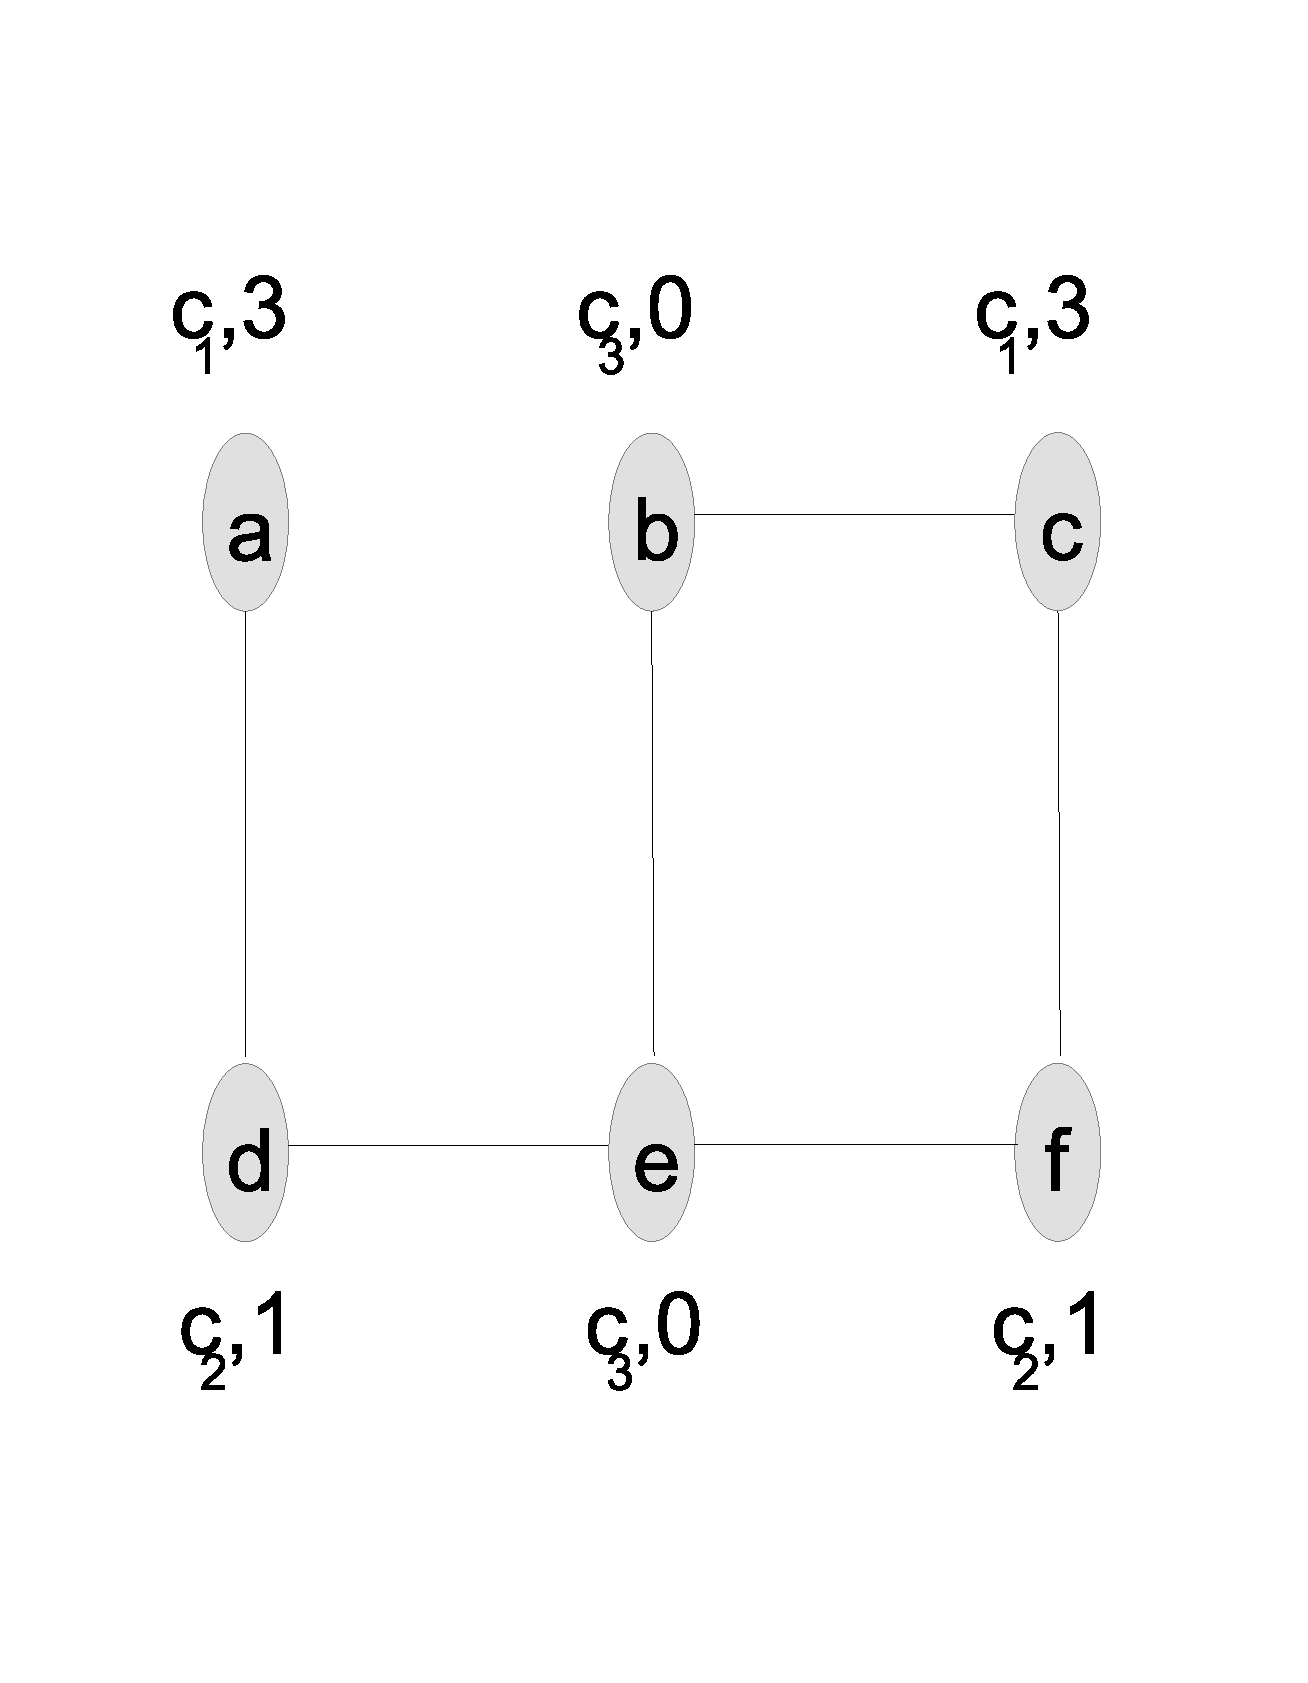
\psfig{file=colors.eps,width=9cm,height=6cm}}
  \caption{ A hypothetical protein interaction network with six nodes
    \{a, b, c, d, e, f\}. The network is colored using three colors
    \{$c_1$, $c_2$, $c_3$\}. Each node carries two labels.  The label
    on the left denotes the color assigned to this node.  The one on
    the right is the node's $k_{max}$ value. For instance node d is
    assigned to color $c_2$ and its $k_{max}$ value is 1 (i.e., there
    is no other node assigned to color $c_2$ within 1-hop of node d). }
  \label{fig:colors}
\end{wrapfigure}


Our key contribution is to establish the relationship among network
topology, node colors and sucess probability.  \ignoreme{ By doing
  this, unlike Scott {\it et al.}~\cite{scott}, we compute a
  probability of success unique to each iteration of color coding
  rather than using the same probability for all iterations.}  In this
section, we build the mathematical model that will help us compute the
probability of success in each iteration.

Assume that we are given a protein interaction network similar to the
one described in Section \ref{introduction}, denoted by $G = (V, E,
w)$, where $w(u, v) = -$log $\lambda(u, v)$. Also assume that the
colors of the nodes are already assigned in the current iteration. We
denote the set of possible colors with $\{c_1, c_2, \ldots, c_m\}$
and denote the color of node $v \in V$ with $c(v)$.

Consider any colorful path with $m$ nodes. The number of ways to
assign colors to the nodes of that path while keeping it colorful is
$m!$. Notice that this is equal to the numerator in Equation \ref{ps}
for probability of success. The denominator in that equation, denoted
by $N_c$, is the total number of ways to color that path regardless of
whether it yields a colorful path or not. Before we discuss how we
compute $N_c$, we describe the following concepts.


\begin{define} {\sc (Simple path)}
  Given a network $G=(V,E)$, a {\em simple path} from $u$ to $v$ ($u$,
  $v \in V$) is an ordering $<v_{1},v_{2}, \dots,v_{k}>$, of a subset
  of the vertices of $G$ such that $v_{1}=u$, $v_{k}=v$,
  $(v_{i},v_{i+1}) \in E$ and no vertex $v_{i}$ is repeated $\forall
  i$, $1 \leq i < k$.
\end{define}

Consider two nodes $u$ and $v$ in $G$. Let $k$ be a positive integer.
We say that $v$ is reachable from $u$ in $k$ hops if there is a simple
path from $u$ to $v$ that contains $k$ edges.


\begin{define}
  {\sc ($k$ neighborhood of a node)}. Let $v \in V$ be a node in $G$,
  and $k$ be a natural number.  We define the $k$ neighborhood of node
  $v$ as the set of nodes in $V \backslash \{v\}$ which are reachable
  from $v$ in $k$ hops of less. We denote this set using notation
  $\Psi_k(v)$.
\end{define}

Figure~\ref{fig:colors} shows an example of a colored network.  In
this example, $\Psi_1(a) = \{d\}$ because the node $d$ is the only
node that is reachable from the node $a$ in 1 hop (or less).
Similarly, $\Psi_1(f) = \{c, e\}$, $\Psi_2(a) = \{d, e\}$ and
$\Psi_2(f) = \{c, e, b, d\}$.  Following definition establishes the
relationship between each node of the network and the rest of the
network based on the colors assigned to all the nodes.

\begin{define}
  {\sc ($k_{max}$ value of a node)}. Let $v \in V$ be a node in $G$.
  The $k_{max}$ value of $v$, denoted with $k_{max}(v)$, is the
  largest valued $k$ neighborhood of $v$ that does not contain a node
  with the same color as $v$. Formally, 
$$
k_{max}(v) = \textrm{argmax}_k \{ \forall u \in \Psi_k(v), c(u) \neq c(v)
\}
$$
\label{dfn:kmax:node}
\end{define}

Figure~\ref{fig:colors} shows the $k_{max}$ values for the nodes in
the network. For example, the colors of all the nodes in $\Psi_1(f) =
\{c, e\}$ are different than the color of $f$. When we expand the
neighborhood of $f$ by one, we get $\Psi_2(f) = \{c, e, b, d\}$. In
this set, $c(d) = c(f) = c_2$.  Therefore $k_{max}(f) = 1$.  Similarly
analysis shows that, $k_{max}(a) = 3$ and $k_{max}(b) = 0$. Next
definition characterizes a simple path of the network.

\begin{define} {\sc ($k_{max}$ configuration of a path)}.  Consider a
  simple path $\Phi = v_1 \rightarrow v_2 \rightarrow \ldots
  \rightarrow v_m$ of $m$ nodes in $G$. The $k_{max}$ configuration of
  $\Phi$ is the vector [$k_{max}(v_1)$, $k_{max}(v_2)$, $\ldots$,
  $k_{max}(v_m)$].
\end{define}

As an example, in Figure~\ref{fig:colors}, the $k_{max}$ configuration
of the path $\Phi = a \rightarrow d \rightarrow e \rightarrow f$ is
[3, 1, 0, 1]. That for $a \rightarrow d \rightarrow e \rightarrow b$ is
[3, 1, 0, 0].



\subsection{Bounding the probability of success tightly}
%\subsection{Bounding the number of colorings tightly}

In this section, we focus on one coloring iteration and describe how
we compute the probability of success in that iteration.
  
Notice that there can be many different color assignments that yield
the same $k_{max}$ configuration for the same path. Also, as we will
show later, the number of possible color assignments to the nodes of a
path can be different for different $k_{max}$ configurations. Indeed,
the $k_{max}$ configuration of a path describes the constraints
imposed on all the nodes of that path about how many alternative
colors can be assigned to them. To understand this better, consider a
hypothetical path with $k_{max}$ configuration = [4, 4, 4, 4]. This is
an extreme case in which we know that no two nodes in the path have
the same color. In this case, we can assign colors in 4! = 24
different ways.  Now consider another extreme case when the $k_{max}$
configuration = [0, 0, 0, 0]. In this case each node may or may not
have the same color as its neighbor, leading to $4^4 =256$ alternative
color assignments.




Analysis of these two extreme examples above show that the the number
of possible color assignments to the nodes of a path can be different
for different $k_{max}$ configurations. However, we need a systematic
and efficient strategy to compute this number for any possible
$k_{max}$ configuration.  To solve this problem, we first build a new
undirected and unweighted graph, called the {\em constraint graph}
from the $k_{max}$ configuration. By utilizing the constraint graph we
transform the problem of finding the number of possible colorings to
the chromatic polynomial computation problem. Next, we describe how we
build the constraint graph.



\begin{figure}[t]
\centering
\subfigure[]{
  \label{maxk:path}
  \includegraphics[width = 0.35\textwidth]{figures/kmax_path}
}
\goodgap
\subfigure[]{
  \label{maxk:graph}
  \includegraphics[width = 0.27\textwidth]{figures/kmax_graph}
}
%\centerline{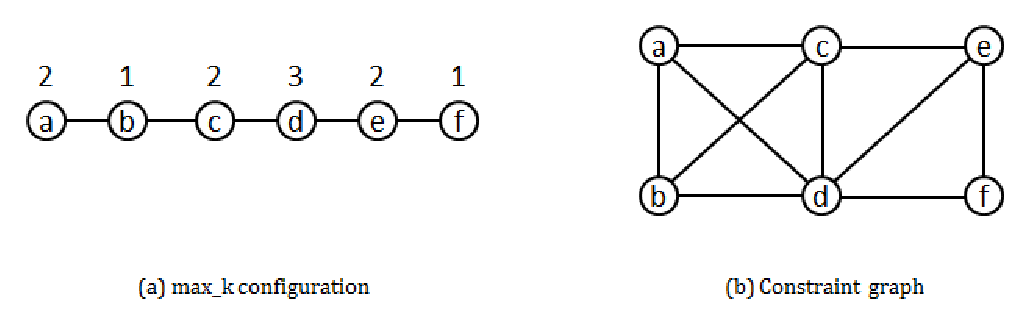
\psfig{file=maxk.eps,width=16.5cm}}
  \caption{(a) An example 6-node path with its $max\_k$ configuration
    shown above it. Each $max\_k$ value translates to the number of
    nodes that have to be of different color on either direction. (b)
    The corresponding constraint graph $W$: each pair of adjacent
    nodes have to be of different color. Finding the value of the
    chromatic polynomial $P(W, m)$ yields the number of coloring
    possibilities for the path under the given constraints.}
  \label{maxk}
\end{figure}

Assume that we are given a simple path $\Phi = v_1 \rightarrow v_2
\rightarrow \ldots \rightarrow v_m$ of $m$ nodes along with its
$k_{max}$ configuration [$k_{max}(v_1)$, $k_{max}(v_2)$, $\ldots$,
$k_{max}(v_m)$]. We build a constraint graph with $m$ nodes \{$u_1$,
$u_2$, $\ldots$, $u_m$\}.  We denote the constraint graph as $W = (H,
L)$ where $H$ is its set of nodes and $L$ is its set of edges.  For
all pair of nodes $u_i$ and $u_j$ in $H$, we draw an undirected edge
between them if the following condition holds:
$$
j - i \leq \max\{k_{max}(v_i), k_{max}(v_j)\}.
$$
Figure~\ref{maxk} shows an example of a path, its $k_{max}$
configuration and the corresponding constraint graph.

Notice that the indices $i$ and $j$ in the above description show the
positions of the nodes on the given path $\Phi$.  As a result, an edge
between $u_i$ and $u_j$ in the constraint graph indicates that $v_i$
and $v_j$ can not be of the same color according to the underlying
$k_{max}$ configuration. Thus, each possible coloring of the given
path $\Phi$ that obeys the $k_{max}$ configuration corresponds to a
chromatic coloring of the constraint graph $W$ and vice versa.


Formally, the value of the chromatic polynomial $A(W, m)$ is equal to
the number of ways of coloring $W$ using $m$ colors without any pair
of adjacent nodes having the same color.  Applying chromatic
polynomials on the constraint graph of a path yields the number of
possible colorings of that path. Closed form formulas of these
polynomials exist in the literature for specific graph topologies,
such as paths, trees, complete graphs and cycles. However, the
constraint graph of a path can have any topology, and thus, these
formulas will not apply for many $k_{max}$ configurations. Therefore,
we use a dynamic programming solution following edge-contraction
recursive rule based on the fundamental reduction theorem~\cite{dong}.
To describe this, we first define two contraction operators on graph
$W$. The first one removes one edge, ($u$, $v$) from the edge set of
$W$. We denote this with $W - (u, v)$. The second one merges two
nodes, $u$ and $v$, into a single node $uv$. To do this, we inserting
a new node $uv$ to $W$ that is adjacent to all the nodes which are
adjacent to either $u$ or $v$. We then remove the nodes $u$ and $v$
along with all the edges incident to them. We denote this merge
operation with $W / \{u, v\}$. Using this notation, the dynamic
programming works by applying the following equation.
\begin{equation}
A(W, m) = A(W - (u, v), m) - A(W / \{u, v\}, m)
\label{eqchromatic}
\end{equation}
The stopping criteria in this equation is the case when $W$ does not
contain any edge (i.e., no more constraints are remaining). In other
words $W = (H, \emptyset)$. In that case, all the nodes can take any
of the $m$ colors, and thus $A(W, m) = m^{|H|}$.  In
Equation~\ref{eqchromatic}, the first term, i.e, $A(W - (u, v), m)$,
formulates the number of chromatic colorings by disregarding the
constraint between $u$ and $v$. The second term, i.e, $A(W / \{u, v\},
m)$ corresponds to the number of colorings in which only the
constraint between $u$ and $v$ violates chromatic coloring of $W$. So,
the difference the difference of these two terms tields the number of
chromatic colorings of $W$.


Now we are ready to compute the probability of success, $P_s$, for a
coloring instance of our method (i.e, Step 6 of Algorithm~\ref{alg1}).
At each iteration, we first build the constraint graph $W$ of the best
colorful path $\Phi$ found at that iteration. We compute the number of
chromatic colorings of $W$ as $A(W, m)$ as described above.  We then
set $N_c = A(W, m)$ and compute the probability of success using
Equation~\ref{ps} as $P_s = m!/N_c = m!/A(W, m)$.


\subsection{Analysis of the probability of success}

We need to answer two key questions regarding how we compute the
probability of success: (i) Is it guaranteed to be better than
existing methods including Scott et al.~\cite{scott} and G{\"u}lsoy et
al.~\cite{gulsoy} and (ii) Is it theoretically sound? In this section,
we discuss these theoretically. We defer the experimental evidence to
Section~\ref{sec:exp}.

To answer the first question, we define a partial order between
$k_{max}$ configuration of a paths as follows: Consider two such
configurations ${\bf x} =$ [$x_1$, $x_2$, $\ldots$, $x_m$] and ${\bf
  y} =$ [$y_1$, $y_2$, $\ldots$, $y_m$]. We say that ${\bf x} \leq
{\bf y}$ if and only if $\forall_i$, $x_i \leq y_i$.

\begin{proposition}
  Consider two $k_{max}$ configurations ${\bf x}$ and ${\bf y}$ of two
  simple paths of $m$ nodes. Let us denote their corresponding
  constraint graphs $W_x$ and $W_y$ respectively.  If ${\bf x} \leq
  {\bf y}$ then $A(W_x, m) \geq A(W_y, m)$.

\label{prop:order}
\end{proposition}

We ommit detailed proof of Proposition~\ref{prop:order} due to space
limitation. However, briefly it follows from the observation that
${\bf x} \leq {\bf y}$ implies that $W_x$ is topologically a
subnetwork of $W_y$. In other words, $W_x$ has only a subset of the
constraints imposed by $W_y$. Thus, the chromatic polynomial 
$A(W_x, m)$ cannot be less than $A(W_y, m)$.

Proposition~\ref{prop:order} has two important implications. First,
traditional color coding method (such as Scott et al.~\cite{scott})
computes $N_c = m^m$. This is the most conservative case in our model
when the $k_{max}$ configuration is [0, $\ldots$, 0].  Clearly, this
will yield the worst (i.e., largest) possible value for the chromatic
polynomial since $[0, $\ldots$, 0] \leq {\bf y}$ for any configuration
${\bf y}$. Second, let $t$ be the smallest $k_{max}$ value among all
the nodes in the network. The formulation by G{\"u}lsoy et
al.\cite{gulsoy} corresponds to $k_{max}$ configuration is [$t$,
$\ldots$, $t$]. Let ${\bf y}$ be the $k_{max}$ configuration of any
$m$-node path in the same network. We have [$t$, $\ldots$, $t$] $\leq
{\bf y}$ since all the entries of ${\bf y}$ have value $t$ or more.
We conclude from these two implications that our method is guaranteed
to produce less or same $N_c$ value as the mentioned existing methods
depending on the network topology and the color distribution.  Smaller
values for $N_c$ implies larger success probability, and thus, faster
convergence to the desired confidence value.




\tk{This is where I left}




{\color {blue} According to this method, the value of $N_c$ for the
  example path shown in Figure \ref{maxk}(a) is 5,760, while Scott et
  al.\cite{scott} and G{\"u}lsoy et al.\cite{gulsoy} would
  respectively yield $N_c$ = 46,656 and 18,750 for the same example.
  Such a decrease in the value of $N_c$ leads to an increase in the
  value of $P_s$ according to equation (\ref{ps}). 
} 


\section{Experiments}
\label{sec:exp}

In this section, we evaluate our method on real datasets. We
implemented our method in Java language. We ran our experiments on Java
runtime environment version 1.6 on Linux machines with 2.2-GHz dual AMD Opteron
dual core processors, and 3 GBs of main memory.

\paragraph{Datasets}
In our experiments, we used two datasets of protein interactions
in Homo Sapiens and Rattus Norvegicus from MINT\cite{mint1} (the Molecular
INTeraction database). The first one is a large dataset of 15472 interactions
among 6122 proteins. The second one is a smaller dataset of 806 interactions
among 631 proteins. Each interaction is described by two interacting proteins and a
reliability score between 0 and 1 that represents the level of confidence that
this interaction truly exists. MINT calculates reliability scores of
interactions using a heuristic formula of available evidence, including the
size and type of the experiment reporting the interaction, sequence similarity
of ortholog proteins and the number of publications supporting the
interaction\cite{mint2}. 

We use the negative logarithm of MINT reliability scores as edge weights. In all
experiments, we find pathways starting within the set of membrane proteins and
ending within the set of transcription factors. We use the Gene Ontology
database\cite{go} to identify membrane proteins and transcription factors of each
dataset. We identify membrane proteins as the ones under the terms GO:0005886
and GO:0004872, and transcription factors as the proteins under the terms
GO:0000988, GO:0001071 and GO:0006351.

\subsection{Performance assessment and comparison}


\begin{figure}[h]
\centering
\subfigure[H.sapiens, path length = 6]{
	\label{iterations_hsa_6}
	\includegraphics{results/iterations/hsa6}
}
\goodgap
\subfigure[H.sapiens, path length = 8]{
	\label{iterations_hsa_8}
	\includegraphics{results/iterations/hsa8}
}
\subfigure[R.norvegicus, path length = 6]{
	\label{iterations_rat_6}
	\includegraphics{results/iterations/rat6}
}
\goodgap
\subfigure[R.norvegicus, path length = 8]{
	\label{iterations_rat_8}
	\includegraphics{results/iterations/rat8}
}
\caption{Confidence level acheived after a given number of iterations,
comparing our method to Scott et al. and empirical confidence. X-axis is the
number of iterations finished, and Y-axis is the level of confidence in the
optimality of the result, for H.sapiens and R.norvegicus at different path
lengths. The empirical line denotes the observed probability that the optimal
path is found at or before a given iteration, averaged over several experiments.}
\label{iterations}
\end{figure}



We run an experiment to measure how fast the value of confidence rises with each
iteration in both our method and the one presented by Scott et al.\cite{scott}.
We run each method for 500 iterations and measure the overall confidence after
each iteration is finished. We also compare these results with the empirical
confidence, which is the probability of finding the optimal pathway as
empirically observed. To compute the empirical confidence, we run 500
coloring iterations and assign each iteration a value $s \in \{0, 1\}$, where
$s = 1$ if the optimal pathway is found in this iteration or in a preceding one,
and $s = 0$ otherwise. We repeat this experiment multiple times and take the
average values of $s$ for each iteration as the empirical confidence of this
iteration. Figure \ref{iterations} shows the confidence value as more iterations
finish, for our method and Scott et al. and also the empirical confidence value.
The figure shows a gap between Scott et al. confidence and empirical confidence,
which is expected because of the conservative way they use to calculate success
probability of an iteration, as discussed in section \ref{background}. This gap
increases as the path length parameter increases. Our method closes this gap and
produces confidence values that are closer to the empirical confidence values.
The figure also shows that our method produces higher confidence values than
Scott et al. for the same number of iterations.

\begin{figure}[h]
\centering
\subfigure[H.sapiens, path length = 6]{
	\label{times_hsa_6}
	\includegraphics{results/times/time_hsa6}
}
\goodgap
\subfigure[H.sapiens, path length = 8]{
	\label{times_hsa_8}
	\includegraphics{results/times/time_hsa8}
}
\subfigure[R.norvegicus, path length = 6]{
	\label{times_rat_6}
	\includegraphics{results/times/time_rat6}
}
\goodgap
\subfigure[R.norvegicus, path length = 8]{
	\label{times_rat_8}
	\includegraphics{results/times/time_rat8}
}
\subfigure[R.norvegicus, path length = 9]{
	\label{times_rat_9}
	\includegraphics{results/times/time_rat9}
}
\caption{Total time needed to acheive a given level of confidence by our method
and Scott et al. X-axis is the level of confidence in the optimality of the
result, and Y-axis is the total time taken to acheive this confidence level,
for H.sapiens and R.norvegicus at different path lengths. Lower values are
better.}
\label{times}
\end{figure}



We also measure the total time taken by our method to reach a given
confidence level as opposed to that of Scott {\it et
  al.}~\cite{scott}. We run both methods for 500 iterations and
measure, after each iteration, the confidence level reached and the
overall time taken by both methods. Figure \ref{times} shows that our
method takes less time than Scott et al. to achieve the same level of
confidence. The figure also shows that the our performance lead
increases as the path length parameter increases.



\subsection{Validation Experiments}
\label{sec:validation}


So far we have shown that our method outperforms existing coloring
strategies in terms of the running time performance. In this section,
we evaluate the biological significance of the results we can find
using our method. 

It is worth mentioning that our method returns the same results as
Scott {\it et al.}~\cite{scott} when both of them are allowed to reach
a high confidence value (such as 99\% confidence). The main difference
is that our method scales to larger networks and longer paths.
Therefore, here we will only focus on the results obtained by our
method.


\subsubsection{Statistical significance of the results}
\label{sec:zscore}

%\begin{wraptable}{r}{0.40\textwidth}
\begin{table}[t]
  \tbl{$Z$-scores calculated for the optimal paths found by our method for
  H.sapiens and R.norvegicus for different path lengths. $Z = \frac{\mu
  - \theta}{\sigma}$ where $\mu$ is the average weight of 1000 randomly
  generated paths, $\sigma$ is their standard deviation, and $\theta$ is the
  weight of the optimal path found by our method.} {
\begin{tabular}{|l|c|c|c|c|c|c|c|c|c|}
\hline
	&	\multicolumn{9}{c|}{Path Length}		\\ \cline{2-10}
Dataset	&	\multicolumn{3}{c|}{6}	&	\multicolumn{3}{c|}{7}	&
	\multicolumn{3}{c|}{8}	\\
	\cline{2-10} 
		&	\begin{math}\mu\end{math}	&	\begin{math}\theta\end{math}	&
	\begin{math}Z\end{math} & \begin{math}\mu\end{math}	&	\begin{math}\theta\end{math}	&
	\begin{math}Z\end{math} & \begin{math}\mu\end{math}	&
	\begin{math}\theta\end{math}	& \begin{math}Z\end{math}	\\ \hline
{\it H.sapiens}	&	5.906	&	0.129	&	5.409	&	7.074	&	0.130	&	5.477	&	8.341	&
0.221	&	5.764	\\
{\it R.norvegicus}	&	4.975	&	4.540	&	0.889	&	7.307	&	5.025	&	1.453	&
8.457	&	4.858	&	1.467
\\
\hline
\end{tabular}
}
\label{tab:zscore}
\end{table}
%\end{wraptable}

In this section we assess the statistical significance of the paths found of our
method; how our results compare to random paths. We use $Z$-score to
measure statistical significance. For each dataset and path length, we run our method to
get the path with the minimum weight $\theta$. we then generate 1000 random
simple paths that start at a membrane protein and end at a transcription
factor. We compute the average weight $\mu$ of these random paths and their
standard deviation $\sigma$. We then compute the $Z$-score as follows
\begin{equation}
Z = \frac{\mu - \theta}{\sigma}
\end{equation}
$Z$-score indicates by how many standard deviations our optimal weight is
better than the weight of an average random path, so higher values are better.
Table~\ref{tab:zscore} shows $Z$-scores for H.sapiens and R.norvegicus for path
length 6, 7 and 8. Our results are always better than the random ones.
The calculated $Z$-scores range from 0.89 to 5.76. It can also be observed that,
for a given dataset, $Z$-score increases with increasing the path length, which
is expected because increasing the size of random selection leads to less
chances of the selected path being better or closer to the optimal path.
From these observations observations, we can infer that our results are
statistically significant.


\subsubsection{Biological significance of the results}

\begin{wrapfigure}{r}{0.50\textwidth}
  \centering
  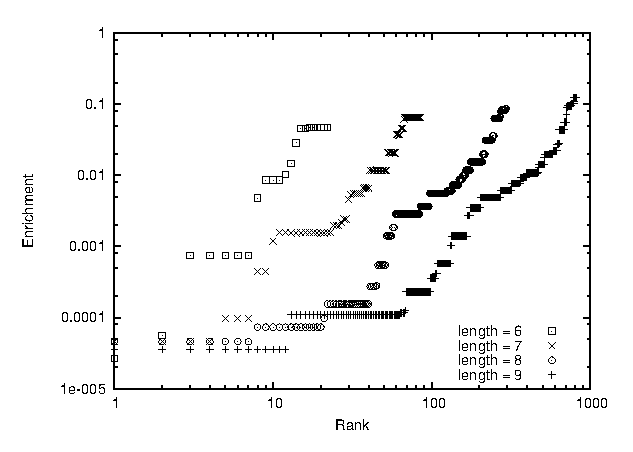
\includegraphics[width=0.45\textwidth]{results/enrichment/enrich-rank}
  \caption{Sorted values of functional enrichment of optimal and suboptimal
  paths found at different iterations of our method. X-axis is the rank of the
  path with regard to its functional enrichment in log scale, and Y-axis is the
  enrichment value of this path. Lower values are better.}
  \label{fig:enrichment-rank}
\end{wrapfigure}


\begin{wrapfigure}{r}{0.50\textwidth}
  \centering
  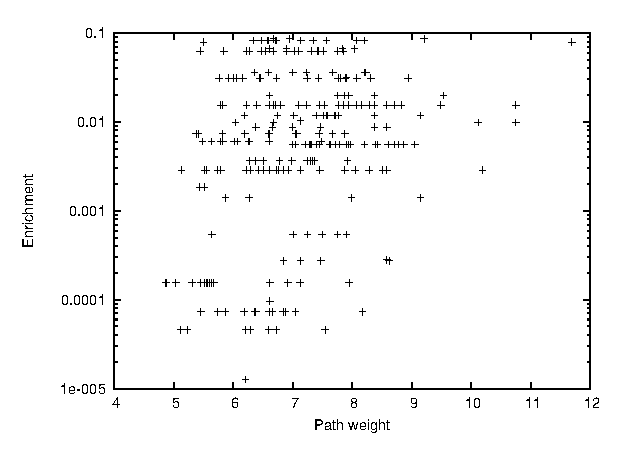
\includegraphics[width=0.45\textwidth]{results/enrichment/enrich-score}
  \caption{Functional enrichment values of paths against their weights. X-axis
  is path's weight and Y-axis is its corresponding enrichment value. Lower
  values are better.}
  \label{fig:enrichment-score}
\end{wrapfigure}


Another important question is: how biologically significant are our results? To
answer this question, we validate our results using functional enrichment. We
use the Gene Ontology\cite{go} to compute functional enrichment of paths found
at different iterations of our method. Let $\Phi$ be the path being tested, $T$
be the universal set of GO terms, $m$ be the path length, $M$ be the total
number of proteins in the dataset, $G_i$ be the total number of proteins
annotated with the Go term $t_i$ in the dataset, and $g_i$ be the number of
proteins annotated with $t_i$ in $\Phi$. We compute functional enrichment of
$\Phi$ as $\min_{t_i \in T} P(X \geq g_i | M, m, G_i)$ where $X$ is a random
variable under under a hypergeometric distribution with these parameters. Lower
values of are better.



 
\subsection{Discussing paths found}
 
 \begin{figure}[h]
\centering
\subfigure[All proteins annotated by GO:0042058 - regulation of epidermal growth
factor receptor signaling pathway]{
	\label{fig:path_go0042058}
	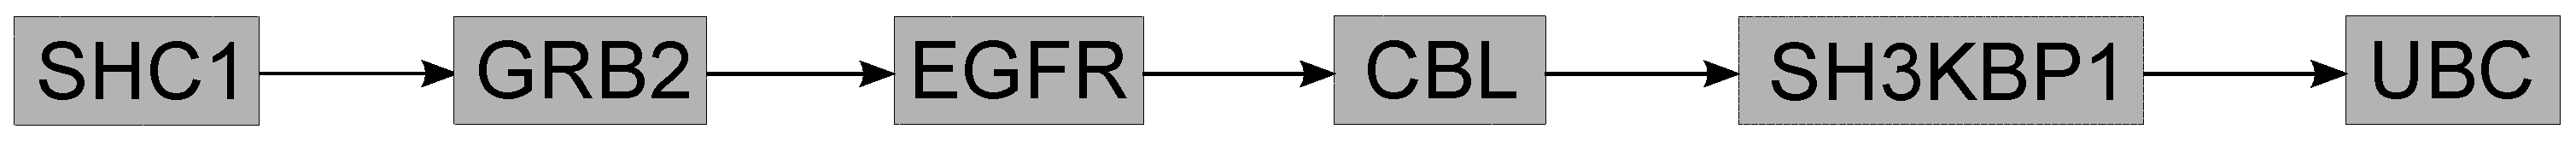
\includegraphics[width = 0.8\textwidth]{figures/path_go0042058}
}
\subfigure[First five proteins annotated by GO:0042059 - negative regulation of
epidermal growth factor receptor signaling pathway]{
	\label{fig:path_go0042059}
	\includegraphics[width = 0.8\textwidth]{figures/path_go0042059_2}
}
\subfigure[All proteins annotated by GO:0046875 - ephrin receptor binding]{
	\label{fig:path_go0046875}
	\includegraphics[width = 0.8\textwidth]{figures/path_go0046875}
}
\caption{Caption goes here}
\label{fig:paths}
\end{figure}
 


\section{Conclusion}
Here goes the conclusion.


\bibliographystyle{ws-procs11x85}
\bibliography{references}

\end{document}